\section{Real EEG Measurements}
Let's look at estimation of active sources, $k$, on the real EEG measurements. 
For this estimation one can not compare the estimation to the real sources as in the previous section.
Instead, one applies the estimation tool, looking for replicas, on the real EEG measurements and makes a conclusion from the observed result.

For the estimation one will only look at one time segment to verify that the estimation of active sources can be applied on real EEG measurements. The estimation will be performed on the S1\_Cclean EEG data set with $\frac{1}{2} M < N$ -- every second sensor is removed. The specification on this data set are $M=13$ and the time segment of interest is $s = 10$. 
For the estimation one must give an initial guess for the number of active sources. Remember that $k>M$ and $k<N$.  
$k = 17$ has been chosen as a choice for how many active sources exists in time segment $s = 10$. 

Figure \ref{fig:eeg_k} visualize the recovered source matrix $\hat{\mathbf{X}}$ from time segment $s=10$ for $M=13$ and $k = 17$.
\begin{figure}[H]
    \centering
	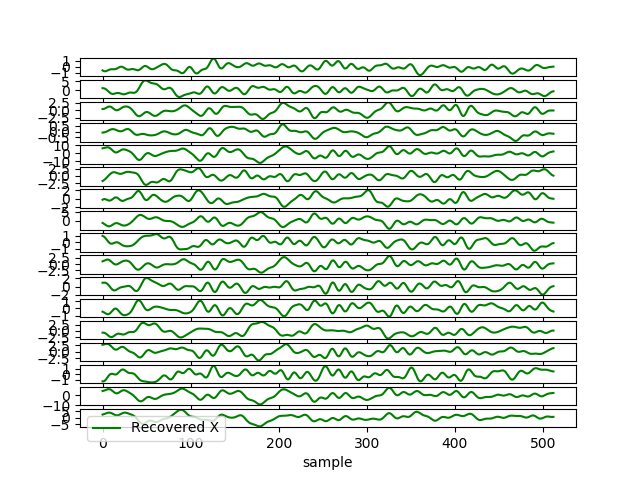
\includegraphics[scale=0.5]{figures/ch_estimate/eeg_k_timeseg_10.png}
	\caption{The recovered source matrix $\hat{\mathbf{X}}$ with $k=17$ active source for the EEG data set with $M=13$.}
	\label{fig:eeg_k}
\end{figure}
\noindent
From figure \ref{fig:eeg_k} one see that all $k$ active sources are visible and there seem not to be any visible indication of a active source being non-active. 

From the list of replicates from figure \ref{fig:eeg_k} only four sources are the 'real' active source while the rest are replicates of those four. The 'real' active sources can be found in row 2, 5, 16 and 17. This leads to the conclusion that for time segment $s=10$ with system specification $M=13$ for the S1\_Cclean EEG data set only have $k=4$ active sources.



